\documentclass[12pt,a4paper,titlepage]{article}
\usepackage[left=2.5cm,text={16cm,20cm},top=4cm]{geometry}
\usepackage[T1]{fontenc}
\usepackage[czech]{babel}
\usepackage[utf8]{inputenc}
% dalsi balicky
\usepackage{graphicx}
\usepackage{enumitem}
\usepackage{indentfirst}
\usepackage{float}
\usepackage{svg}
\usepackage{amsmath}
\usepackage{url}
\usepackage{graphics}
\usepackage{graphicx}
\usepackage{multicol}
\usepackage{color}
\graphicspath{ {images/} }
\usepackage[bookmarksopen,colorlinks,plainpages=false,urlcolor=blue,
unicode,linkcolor=black]{hyperref}

\bibliographystyle{czplain}

%úvodzovky
\providecommand{\uv}[1]{\quotedblbase #1\textquotedblleft}

\begin{document}

\begin{titlepage}
\begin{center}
    {
    	\Huge\textsc{Vysoké učení technické v~Brně}}\\
    \smallskip
    {
    	\huge\textsc{Fakulta informačních technologií}}\\
    \bigskip
    \vspace{\stretch{0.382}} %pomery odpovedajúcí zlatému rezu
    \huge{Mikroprocesorové a vestavěné systémy}\\
    \smallskip
    \Huge{Hra Life (celulární automat) na maticovém displeji}\\
    \vspace{\stretch{0.618}}
\end{center}
    {\Large \today \hfill David Kozák (xkozak15)  }\\
    \smallskip
\end{titlepage}

\newpage
\tableofcontents
\newpage

\section{Úvod}
Tato dokumentace popisuje projekt do předmětu IMP, který v roce 2016 vytvořil student třetího ročníku FIT VUT David Kozák. V rámci projektu byl navržen a naimplementován projekt pro FITKIT\ref{fitkit} pracující s maticovým displayem modelujícím základní pravidla hry Life\ref{game-of-life}. Hlavním úkolem v tomto projektu vytvořit řídící program pro mikrokontrolér msp430\ref{msp430}, který je součástí fitkitu.
\section{Popis ovládání a implementace}
Tato sekce tvoří jádro celé dokumentace, čtenář zde nalezne jak popis ovládání výsledné aplikace, tak i důležité technické detaily.
\subsection{Popis ovládání}
Celý projekt se ovládá za pomoci tlačítek, která jsou součástí fitkitu. Pro účely této sekce stačí následující znázornění.

\begin{minipage}{\linewidth}
\bigskip
\begin{center}
  \begin{tabular}{ | l | c | r | l |}
    \hline
    \textcolor{red}{1} & \textcolor{red}{2} & \textcolor{red}{3} & A \\ \hline
    4 & 5 & 6 & B \\ \hline
    7 & \textcolor{red}{8} & \textcolor{red}{9} & \textcolor{red}{C} \\ \hline
    * & \textcolor{red}{0} & \textcolor{red}{\#} & D \\
    \hline
  \end{tabular}
  \captionof{figure}{Klávesnice na fitkitu} \label{fitkit:keyboard}
\end{center}
\bigskip
\end{minipage}


Jejich skutečnou podobu lze vidět na obrázku[\ref{foto}] v následující sekci popisující schéma zapojení zapojení. Klávesy označené červenou barvou jsou využity pro ovládání aplikace, klávesy zobrazené černou barvou se momentálně nevyužívají.

Klávesy \textit{1,2,3} slouží pro zobrazení třech počátečních konfigurací, které jsou nastaveny přímo v kódu. Při stisknutí jednoho z těchto tlačítek se současné zobrazování zastaví a dojde k načtení příslušného výchozího stavu.

Klávesy \textit{0} a \textit{\#} slouží pro ovládání běhu aplikace. Klávesa \textit{0} funguje jako \textit{pause/play}. Klávesa \textit{\#} slouží v režimu pause jako tlačítko pro krokování, které posune hru o jeden krok vpřed.

Klávsesy \textit{8} a \textit{9} slouží pro přepínání mezi režimem 8-mi okolí a 9-ti okolí. Rozdíl mezi těmito módy spočívá v tom, že v 9-ti okolí je do okolí buňky počítána i buňka samotná.

Většina výše zmíněných kláves též jako vedlejší jev vypíše nějaký text na LCD display kitu. Pro smazání totoho texto slouží klávesa \textit{C},která vymaže obsah displaye.

\subsection{Schéma zapojení}
Maticový display je připojen přímo na porty mikrokontroléru. Ten jej přes tyto porty ovládá. Zapojení můžete vidět v následující tabulce. 

\begin{minipage}{\linewidth}
\bigskip
\centering
  \begin{tabular}{ | l | l|}
    \hline
    Řádek & Port \\ \hline
    0 & P6M0 \\ \hline
    1 & P6M1  \\ \hline
    2 & P6M2 \\ \hline
	3 & P6M3 \\ \hline
	4 & P6M4 \\ \hline
	5 & P6M5 \\ \hline
	6 & P6M6 \\ \hline
    7 & P6M7  \\
    \hline
  \end{tabular}
  \begin{tabular}{ | l | l|}
    \hline
    Sloupec & Port \\ \hline
    0 & P4M0 \\ \hline
    1 & P4M1  \\ \hline
    2 & P4M2 \\ \hline
	3 & P4M3 \\ \hline
	4 & P4M4 \\ \hline
	5 & P4M5 \\ \hline
	6 & P1M4 \\ \hline
    7 & P2M5  \\
    \hline
  \end{tabular}
  \captionof{figure}{Připojení portů na display} \label{fitkit:display}

\bigskip
\end{minipage}

Jelikož displej nabízí možnost svítit dvěma různými barvami a není z dokumentace přesně definován přesný význam všech 24  pinů, bylo potřeba experimentálně ověřit, jak displej funguje, a přiřadit jednotlivým pinům jejich význam. Z dvou možných barev zvolil autor červenou pro její větší výraznost. Výsledné znalosti o displeji můžete vidět na následujícím obrázku, \textit{C} značí sloupce, \textit{R} značí řádky.

\begin{figure}[h]
\centering
\includegraphics[scale=0.5]{display}
\captionof{figure}{Popis využitých portů displaye, černá úsečka značí stěnu, na které je napsán typ displaje} \label{display}
\end{figure}



Pro větší názornost jsou též přiloženy dva obrázky samotného zapojení.

\begin{figure}[h]
\centering
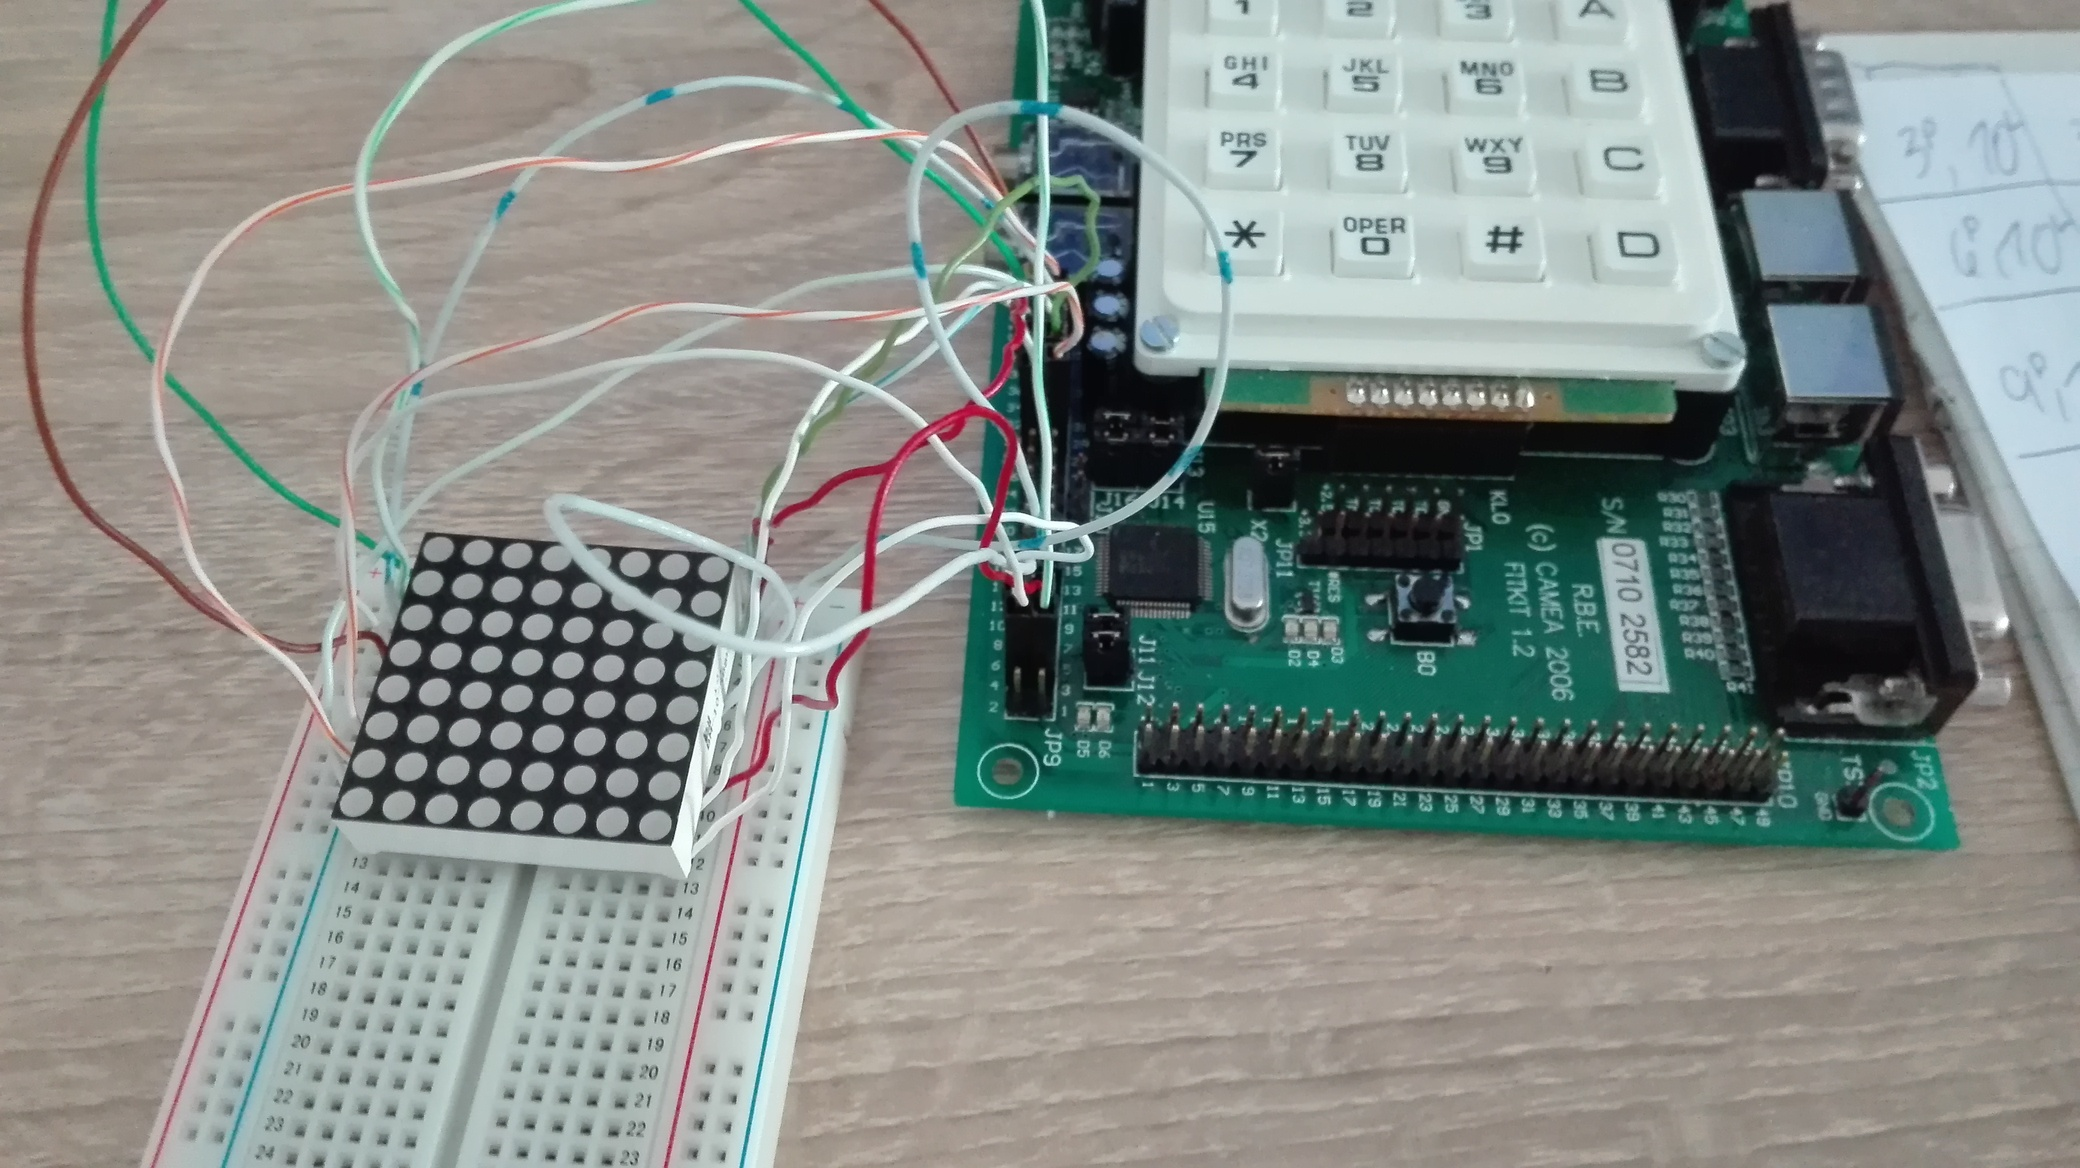
\includegraphics[scale=0.2]{fitkit_resized}
\captionof{figure}{Příklad skutečného zapojení} \label{foto}
\end{figure}

\begin{figure}[h]
\centering
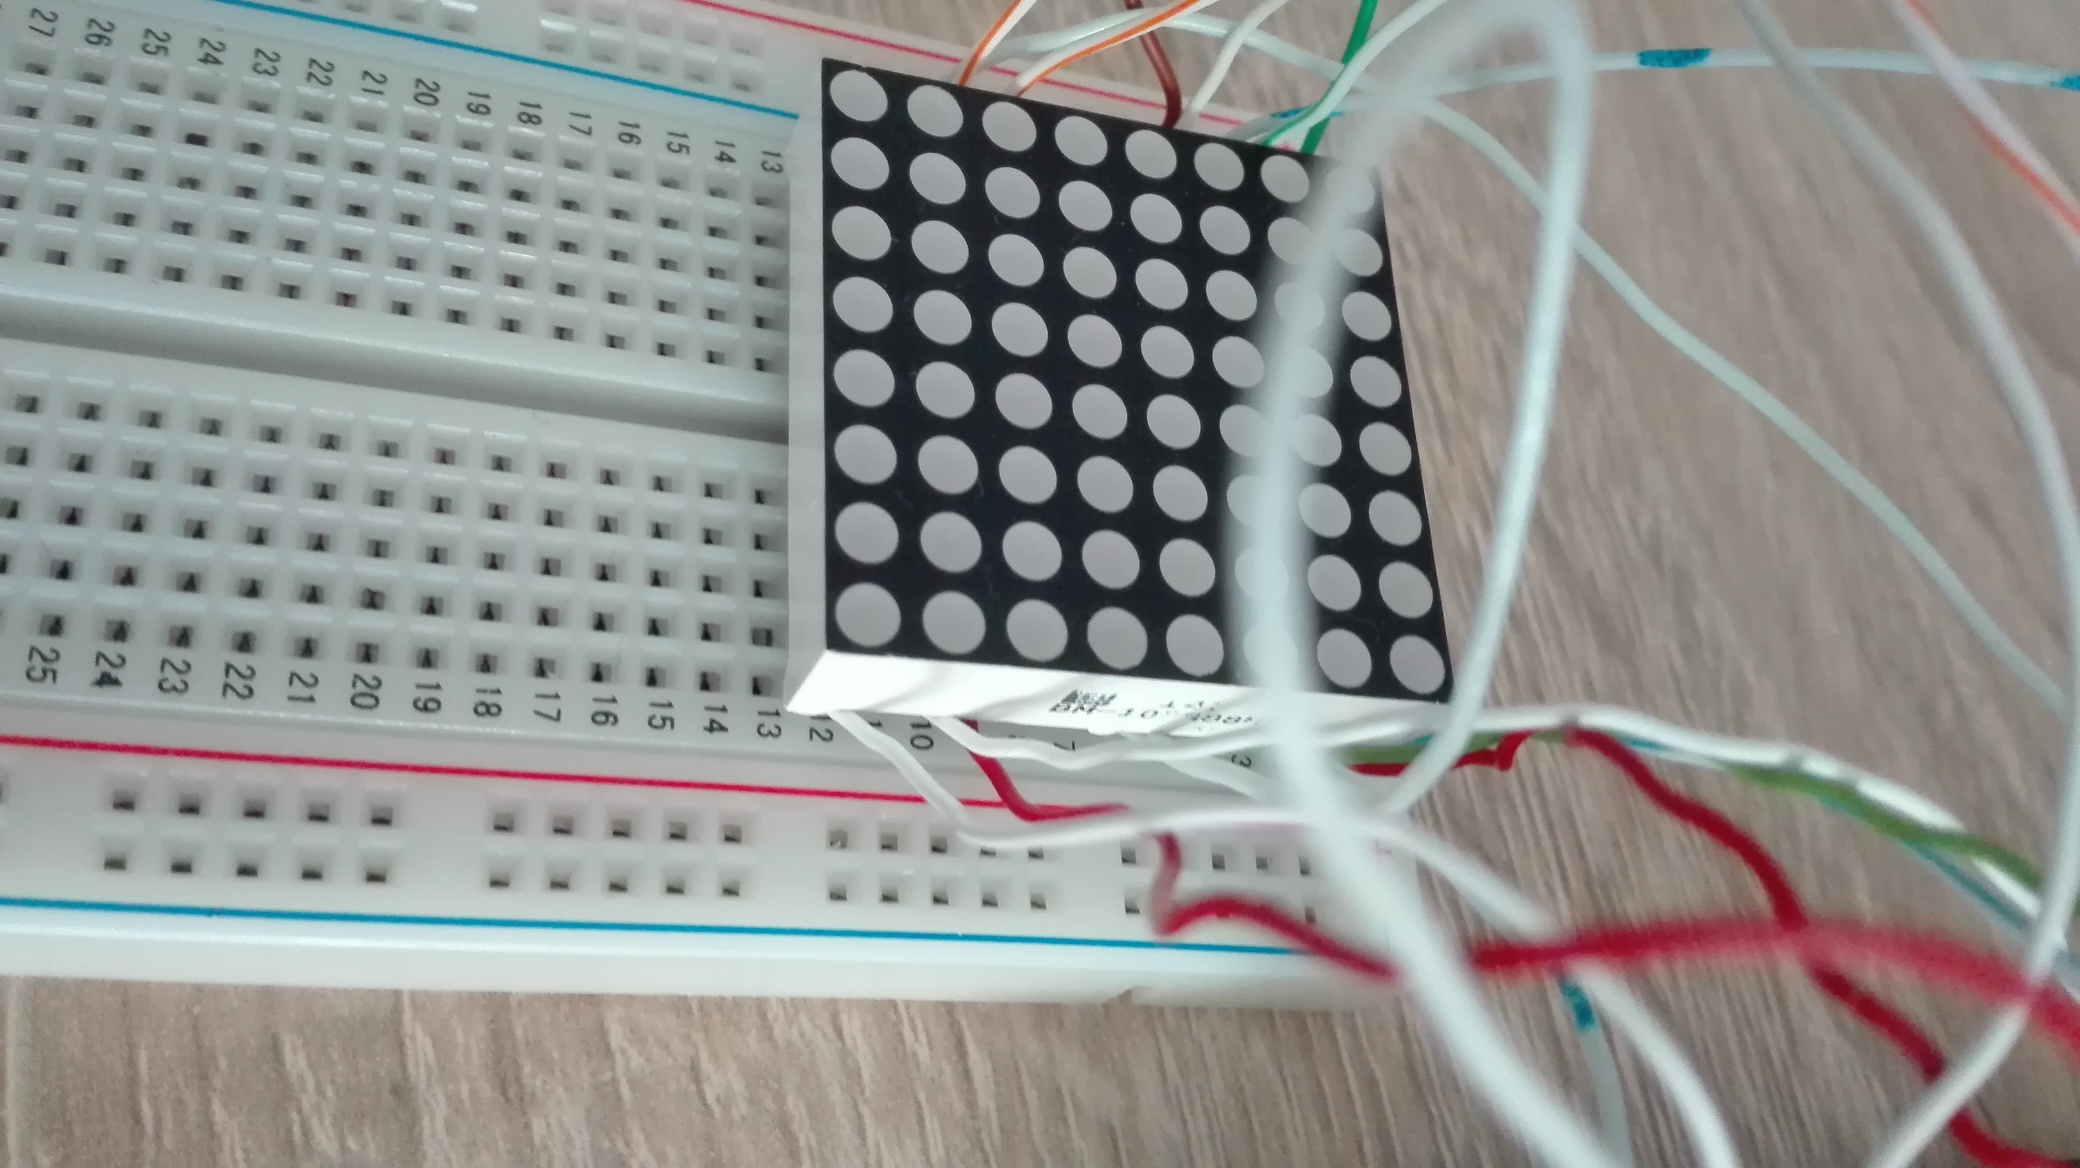
\includegraphics[scale=0.2]{fitkit2_resized}
\captionof{figure}{Příklad skutečného zapojení - detail na displaj} \label{foto2}
\end{figure}

\subsection{Popis způsobu řešení}
Stav programu je uchováván v globálních proměnných. Nejdůležitější proměnné jsou pole 8x8 \textit{cells} reprezentující současný stav a také proměnná boolovského typu \textit{isRunning} určující, zda se simulace má sama chýbat kupředu či nikoliv. Hlavní funkce main nainicialuzuje mcu i fpga a povolí přerušení od časovače. Následně také vybere defaultní výchozí konfiguraci pro hru a přejde do nekonečné smyčky, ve které obsluhuje terminál, klávesnici a také ovládá displej.

Řízení běho programu je prováděno s využitím přerušení. Využívá se přerušení od časovače, které je generováno s frekvencí XYZ Hz a které v případě, že proměnná \textit{isRunning} má hodnotu \textit{true}, vypočítá novou generaci a výsledek uloží do \textit{cells}.


Pokud byla stistknuta klávesa, která má v aplikaci definovaný význam, je provedena rutina ošetřující stisk dané klávesy.
Stisknutí klávesy \textit{0} pouze invertuje hodnotu proměnné \textit{isRunning}, čímž zastaví či spuustí automatické posunování vpřed. Stiskutí klávesy \textit{\#} v režimu \textit{pause} provede posunutí o jeden krok vpřed. Klávesy \textit{1,2,3} bez ohledu na situaci nastaví \textit{isRunning} na false a poté načtou příslušnou počáteční konfiruraci do \textit{cells}.

Klávesy \textit{8} a \textit{9} umožnují přepínat mezi 8-mi okolím a 9-ti okolím .

Samotné vypočítání nové generace probíhá dvouprůchodově. V prvním průchodu dojde k výpočtu nových hodnot do pomocné tabulky, v druhém průchodu se tyto hodnoty přepíší do hlavní tabulky.

\section{Závěrečné shrnutí}
V tomto projektu byla implementována hra Life(celuární automat) s využitím fitkitu a externího maticového displeje. Projekt obsahuje tři výchozí kofigurace, běh je možno pozastavit a krokovat. Ze zadání byly splněny všechny body. Jako možné rozšíření se jeví například možnost ovládat aplikaci z terminálu, konkrétně autor navrhuje možnost pomocí speciálního příkazu zvolit počáteční konfiguraci. Vzhledem k časovému presu ovšem toto rozšíření nebylo implementováno. Demonstraci projektu můžete vidět na videích \ref{video9neighbour} a \ref{video8neighbour}.


\section*{Reference}
\begin{enumerate}[label={[\arabic*]}]
\item Webové stránky projektu FITKIT [cit. 2016-12-09][Online] \\
     \href{https://http://merlin.fit.vutbr.cz/FITkit/}
          {https://http://merlin.fit.vutbr.cz/FITkit/}
     \label{fitkit}
\item Popis hry Game Of Life [cit. 2016-12-09] [Online] \\
    \href{https://en.wikipedia.org/wiki/Conway's\_Game\_of\_Life}
         {https://en.wikipedia.org/wiki/Conway's\_Game\_of\_Life}
    \label{game-of-life}
\item Uživatelský manuál mikrokontroléru MSP430 [cit. 2016-12-09] [Online] \\
    \href{http://www.ti.com/lit/ug/slau144j/slau144j.pdf}
         {http://www.ti.com/lit/ug/slau144j/slau144j.pdf}
    \label{msp430}
\item Ukázka módu 9-ti okolí [cit. 2016-12-09] [Online] \\
    \href{https://www.youtube.com/watch?v=oLCLrJIVXTk}
         {https://www.youtube.com/watch?v=oLCLrJIVXTk}
    \label{video9neighbour}
\item Ukázka módu 8-ti okolí [cit. 2016-12-09] [Online] \\
    \href{https://www.youtube.com/watch?v=EAMCaPm-iR4}
         {https://www.youtube.com/watch?v=EAMCaPm-iR4}
    \label{video8neighbour}
\end{enumerate}
\end{document}
